\documentclass[main.tex]{subfiles}

\begin{document}
\subsection{Workload with many concurrent non-conflicting read-only transactions}

\subsubsection{Problem Analysis}
본 DBMS의 \texttt{Lock Manager}의 구현에서는 \textbf{non-conflicting read-only transactions}가 동시에 수행된다면 
모든 lock 요청에 대해 lock acquire method에서 HashTableEntry를 만들고 바로 lock을 요청자에게 줄 것이다.
모든 요청이 non-conflict이기 때문에 요청마다 HashTableEntry의 수정과 lock acquire 조건 확인은 \emph{불가피}하고 deadlock detection 등의 부가적인 작업을 전혀 하지 않기 때문에
추가로 최적화할 여지는 없다 사료된다. 따라서 더 나아가 아예 concurrency control을 일시적으로 끄는 방법을 고민해볼 필요가 있다.
또한 일반적으로 DBMS는 어떠한 workload가 들어올지 알 수 없기 때문에 DBMS가 read-only transactions인지 알기 위한 수단도 필요하다.
\\

일반적인 상황에서는 conflicting operations가 수행돼 database file의 correctness가 깨질 위험이 있어
이를 방지하고자 concurrency control을 사용하는 것이다. 그러나 read-only transactions이기 때문에 correctness가 깨질 염려는 없다.

\subsubsection{Solution}
\paragraph{(1)}
DBMS가 workload의 성격을 알 수 없는 문제는 \texttt{DBMS API Layer}의 \texttt{trx\_begin}의 인자에 read-only flag를 추가해줌으로써 해결할 수 있다.
다만, read-only로 생성된 transaction에서 write operations를 수행할 경우 해당 operation은 실패하도록 할 필요가 있다.

\paragraph{(2)}
\texttt{Transaction Manager}에서는 non read-only transaction의 개수를 관리해야 한다. 만약 non read-only transaction이 존재한다면 \texttt{Lock Manager}의 기능을 전부 사용하도록 하며
없다면 \texttt{Transaction Manager}에서 \texttt{Lock Manager}를 호출하지 않도록 하면 된다.
현재 DBMS 구조상으로 Transaction Manager에서 Lock Manager에게 lock acquire를 요청하게 되어있으니, 이러한 작업은 \texttt{Transaction Manager}에서 진행하면 된다.
\texttt{Lock Manager}가 transaction에 대해 알 필요가 없다는 점에서 layered architecture violation이 일어나지 않는다.
\\

그러나 단순히 이러한 방식으로 한다면 read-only transactions만 수행하다가 conflicting operations가 들어오는 상황에 대해 대비가 충분하지 않다.
이런 경우에는 non read-only transaction에 대해서만 전체 transaction의 개수를 체크해 transaction의 수가 모두 줄어들 때까지 대기하도록 하면 된다.

\paragraph{(3)}
위 방법을 안전하게 구현하기 위해서는 개수를 담고 있는 변수에 대해 thread safety를 보장해야 한다. 따라서 각 변수를 \textbf{std::atomic}을 이용해 만들어야 한다.
\\

\noindent 따라서 위 방법론을 모두 적용하여 \texttt{Transaction Manager}를 수정한다면 다음과 같다.

\newpage
\begin{figure}[!hbt]
	\centering
	\subfloat[Optimized Transaction]{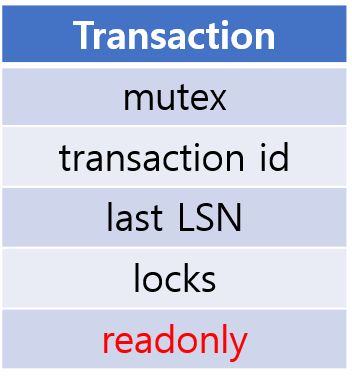
\includegraphics[width=0.4\linewidth]{images/analysis/transaction_edited.png}}
	\subfloat[Optimized Transaction Manager]{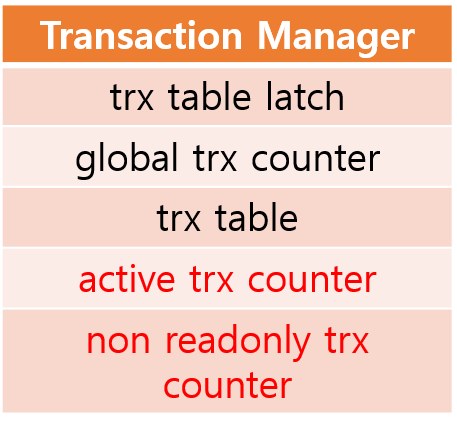
\includegraphics[width=0.4\linewidth]{images/analysis/trx_manager_edited.png}}
	\caption{Optimized \texttt{Transaction Manager}}
\end{figure}

\begin{algorithm}
	\caption{Optimized lock acquire in \texttt{Transaction Manager}}
	\begin{algorithmic}
		\Function{Transaction.LockAcquire}(table id, page id, offset, lock type)
			\If {readonly AND TrxManager.NonReadonlyTrxCounter is 0}
				\State TrxManager.ActiveTrxCounter $\gets$ TrxManager.ActiveTrxCounter $+ 1$
				\State \Return {Acquired}
			\EndIf
			
			\State lock := LockManager.LockAcquire(trx id, table id, page id, offset, lock type)
			
			\If {$\neg$readonly AND lock is Acquired AND TrxManager.ActiveTrxCounter $> 0$}
				\State lock.Wait()
				\Comment{Maybe there are readonly transactions}
			\EndIf
			
			\State LockList += lock
			\State \Return {LockStatus}
		\EndFunction
	\end{algorithmic}
\end{algorithm}

\subsubsection{Correctness}
\noindent \texttt{Lock Manager}를 사용하지 않아도 correctness가 유지되는지 확인할 필요가 있다.

\paragraph{(1)}
Read-only flag를 set 한 뒤 workload with non-conflict read-only transactions를 수행하는 경우에는 conflicting operations가 존재하지 않음으로 이 경우에는 correctness를 해치지 않는다.

\paragraph{(2)}
일반적인 상황에서는 read-only flag가 set 되지 않음으로 원래대로 \texttt{Lock Manager}를 이용하므로 correctness를 해치지 않는다.

\paragraph{(3)}
Read-only flag가 unset인 transactions가 수행되는 도중에 read-only flag가 set 된 transaction이 수행되는 경우에는 non read-only transaction counter가 0이 아니므로 read-only flag가 set 된 transaction이더라도 \texttt{Lock Manager}를 이용하므로 correctness를 해치지 않는다.

\paragraph{(4)}
Read-only flag가 set 된 transactions가 수행되는 도중에 read-only flag가 unset 된 transaction이 수행되는 경우에는 active transaction counter가 0이 아니므로 non read-only transaction이 대기하게 되어 conflicting operations가 수행되지 않아 correctness를 해치지 않는다.


\subsection{Workload with many concurrent non-conflicting write-only transactions}

\subsubsection{Problem Analysis}
일반적인 상황과 대비했을 때 \textbf{non-conflicting write-only transactions}에 대한 workload에 대해서는 \texttt{Buffer Management Layer}의 latch에 의한 wait보다는
\texttt{Lock Manager}의 latch에 의한 wait 시간이 더 길 것이다.
따라서 \texttt{Lock Manager}에 의한 wait 시간을 줄이면 성능 향상을 기대할 수 있을 것이다.
현재 구현된 \texttt{Log Manager}는 mutex를 이용해 lock, unlock으로 \texttt{Log Manager}를 보호한다.
그러나 만약 log buffer가 충분히 커서 buffer의 크기 변경이 자주 일어나지 않음이 보장된다면
mutex로써 \texttt{Log Manager} 전체를 보호할 필요는 LSN을 sequential 하게 발급하기 위함을 제외하면 없다.

\subsubsection{Solution}

\paragraph{(1)}
현재 \texttt{Log Manager}에서 LSN을 발급하는 기준은 Log record file의 header에 존재하는 NextLSN이다. 따라서 해당 변수를 atomic 하게 만들어 전체 LSN의 발급의 thread-safety를 보장할 수 있다.

\paragraph{(2)}
현재 \texttt{Log Manager}는 각 log record를 discrete 하게 저장한다. 하지만 새로운 방식을 적용한다면 마치 file에 적는 것처럼 log를 append 할 수 있도록 log buffer를 수정해야 한다.
따라서 충분히 크게 Log object의 배수 크기만큼 buffer를 만들어야 한다.
또한 현재 \texttt{Log Manager}에는 어디까지 log record file에 저장되었는지 표시하는 flushedLSN이 없다. 하지만 이러한 방법을 사용하려면 추가가 필요하다.

\begin{figure}[!hbp]
	\centering
	\subfloat[Original Log Buffer]{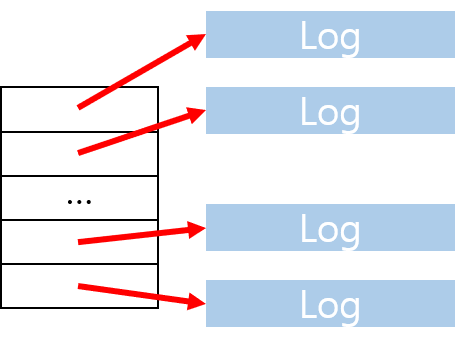
\includegraphics[width=.3\linewidth]{images/analysis/log_current.png}}\hspace{10px}
	\hspace{10px} \subfloat[Edited Log Buffer]{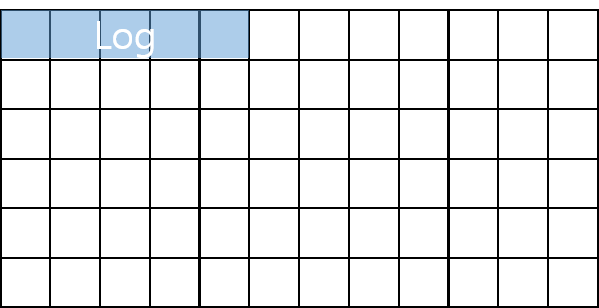
\includegraphics[width=.3\linewidth]{images/analysis/log_edited.png}}
	\caption{Log Buffer Design}
\end{figure}

\paragraph{(3)}
적절히 크게 log buffer의 크기를 잡아도 상황에 따라 크기가 부족해질 수 있다.
이러한 경우에는 mutex 혹은 atomic flag 등을 이용하여 \texttt{Log Manager}를 보호한 채로 log buffer의 크기를 늘려야 한다.
이러한 작업엔 큰 overload가 걸리지만, 충분히 큰 크기이므로 이러한 경우는 비교적 적게 생길 것이다.


\subsubsection{Correctness}
\noindent \texttt{Log Manager}의 latch를 사용하지 않아도 correctness가 유지되는지 확인할 필요가 있다.

\paragraph{(1)}
LSN은 atomic operation을 지원하는 type이므로 LSN을 thread-safe하고 sequential 하게 발급하는데 아무런 문제가 발생하지 않는다.

\paragraph{(2)}
각 log가 발급받은 LSN은 항상 서로 다름이 \textbf{(1)}에 의해 보장되므로 LSN을 바탕으로 log buffer에 접근하여 log를 append 한다면 문제가 발생하지 않는다.

\end{document}
